\chapter{Vérification par mesure des temps à l'oscilloscope}

Cette annexe vient présenter les mesures réaliser

\section{Avec la communication en UART}
\subsection{Mesure avec les 4 inducteurs}
\subsection{Mesure avec les inducteurs 1&2}
\subsection{Mesure avec les inducteurs 3&4}

\section{Sans la communication en UART}
\subsection{Mesure avec les 4 inducteurs}
\subsection{Mesure avec les inducteurs 1&2}
\subsection{Mesure avec les inducteurs 3&4}

\begin{figure}[H]
    \centering
    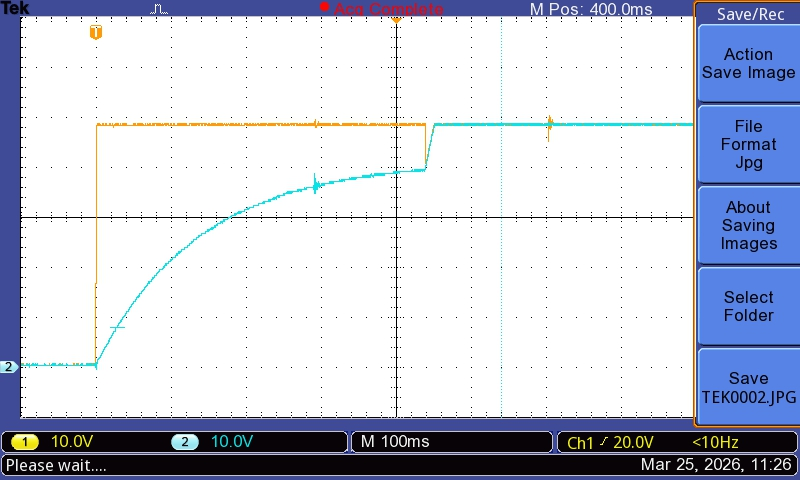
\includegraphics[width=1\linewidth]{Image/Chap.3/MesureCondoCan.JPG}
    \caption{Résultat de la mesure du condensateur personnel}
    \label{fig:ResCanCapa}
\end{figure}
